\section{Auswertung}
\label{sec:Auswertung}

Die Auswertung wurde mit Hilfe eines Programms in Python unter Verwendung der Pakete \texttt{numpy}\cite{numpy} für numerische Rechnungen,
 \texttt{matplotlib}\cite{matplotlib} für die graphische Darstellung und \texttt{uncertainties}\cite{uncertainties} für die Fehlerrechnung ausgeführt.
Die tatsächliche Fehlerberechnung erfolgt durch das Programm, welches auf der Gaußschen Fehlerfortpflanzung beruht.
Im Folgenden werden für die Auswertung im Wesentlichen Produkte der Form
\begin{equation*}
  f(x_1,\ldots,x_n) = \prod_{i=1}^n x_i
\end{equation*}
berechnet, wobei $x_1,\ldots,x_n$ fehlerbehaftete Größen sind.
Dann hat die Größe $f$ den Fehler
\begin{equation*}
  \Delta f = f(x_1,\ldots,x_n) \cdot \sqrt{\sum_{i=1}^n \left(\frac{\Delta x_i}{x_i}\right)^2}
\end{equation*}
und für Summen, die insbesondere bei der Mittelung verwendet werden, also für Funktionen vom Typ
\begin{equation*}
  g(x_1,\ldots,x_n) = \sum_{i=1}^n x_i
\end{equation*}
ist der Fehler
\begin{equation}
  \Delta g = g(x_1,\ldots,x_n) \cdot \sqrt{\sum_{i=1}^n \left(\Delta x_i\right)^2}.
  \label{eq:fehlerDesMittelwertes}
\end{equation}

Die Fehler der einzelnen Messwerte hängen von der jeweiligen Messmethode ab.
Bei jeglicher Zeitmessung wurde eine Abweichung von \qty{0.2}{\second} gewählt.
Diese Wahl nimmt eine mögliche Ungenauigkeit des Ablesens durch das menschliche Auge jeglicher Messwerte an.
Auch wenn der Wert zuerst willkürlich erscheint, wurde durch eine mehrfache Messung der Reaktionszeit zwischen Abschließen des Messintervalls und
Ablesen der Vakuummessgeräte eine großzügige Obergrenze angenommen. Nach 10 unabhängigen Messungen wurde höchstens eine Abweichung von einem Zehntel plus mehreren Hundertsteln Sekunden festgestellt.
Die Fehlerwerte der Messergebnisse im Zusammenhang der Drehschieberpumpe folgen aus der Messungenauigkeit des verwendeten kombinierten Piezo-/Pirani-Sensors.
Im Druckbereich von \num{1200} bis \qty{10}{\milli\bar} liegt sie bei \qty{0.3}{\percent} und von \num{10} bis \qty{2e-3}{\milli\bar} bei \qty{10}{\percent}\cite{sample}.
Dahingegen folgen sie bei den Messungen zur Turbomolekularpumpe aus der Messungenauigkeit des verwendeten kombinierten Pirani-/Kalthkatoden-Sensors.
Diese liegt bei \qty{30}{\percent} im gesamten relevanten Druckbereich \cite{sample}.
Im Folgenden werden für jegliche Messungen beider Pumpen, auch Start-/ und Enddruck, die Fehlerwerte aus diesen Angaben berechnet.

\subsection{Drehschieberpumpe}
    Zur Auswertung wurde das Rezipientenvolumen $V_0 = \SI{34(3.4)}{\liter}$\cite{sample}, der Enddruck $p_E = \qty{6.7(7)e-3}{\milli\bar}$
    und der Startdruck $p_0 = \qty{1000(0.3)}{\milli\bar}$ benutzt.

    \subsubsection{Evakuierungskurve}

    In \autoref{tab:drehEvac} sind die Messergebnisse aufgelistet. Der Mittelwert $p$ dieser Messreihe und der logarithmische Ausdruck
    $\ln\left(\frac{p-p_E}{p_0-p_E}\right)$, dessen Fehler sich mit dem Fehler des Mittelwertes $\sigma_p$ (Gl. \refeq{eq:fehlerDesMittelwertes}) explizit durch \autoref{eq:ln} ausrechnen lässt, sind in \autoref{tab:drehEvacMean} aufgeführt.
    \begin{equation}
        \sigma_{ln} = \sqrt{\left(\frac{\sigma_p}{p-p_E}\right)^2+\left(\frac{\sigma_{p_0}}{p_0-p_E}\right)^2+\left(\frac{(p-p_0)\cdot\sigma_{p_E}}{(p-p_E)(p_0-p_E)}\right)^2}
        \label{eq:ln}
    \end{equation}
    Durch eine lineare Ausgleichsrechnung 
    \begin{equation*}
        \ln\left(\frac{p-p_E}{p_0-p_E}\right) = a_i \cdot t + b
    \end{equation*}
    an die drei Abschnitte des Ausdrucks ergeben sich folgende Parameter:
    \begin{align*}
        a_1 &= \qty{-0.03152(13)}{\per\second} & b_1 &= \num{-0.049(12)} \\
        a_2 &= \qty{-0.0107(4)}{\per\second} & b_2 &= \num{-4.14(12)} \\
        a_3 &= \qty{-0.00424(6)}{\per\second} & b_3 &= \num{-6.349(27)}
    \end{align*}
    Die zugehörigen Ausgleichsgeraden sind in \autoref{fig:drehEvac} eingezeichnet.

    Nach Umstellen von \autoref{eq:evacSaug} und mit Einsetzen von $a_i$ für $\frac{dp}{dt}$
    lässt sich das Saugvermögen abschnittsweise berechnen zu:
    \begin{align*}
        S_1 &= \qty{1.07(11)}{\liter\per\second} \\
        S_2 &= \qty{0.37(4)}{\liter\per\second} \\
        S_3 &= \qty{0.144(14)}{\liter\per\second} 
    \end{align*}

    \begin{figure}
        \centering
        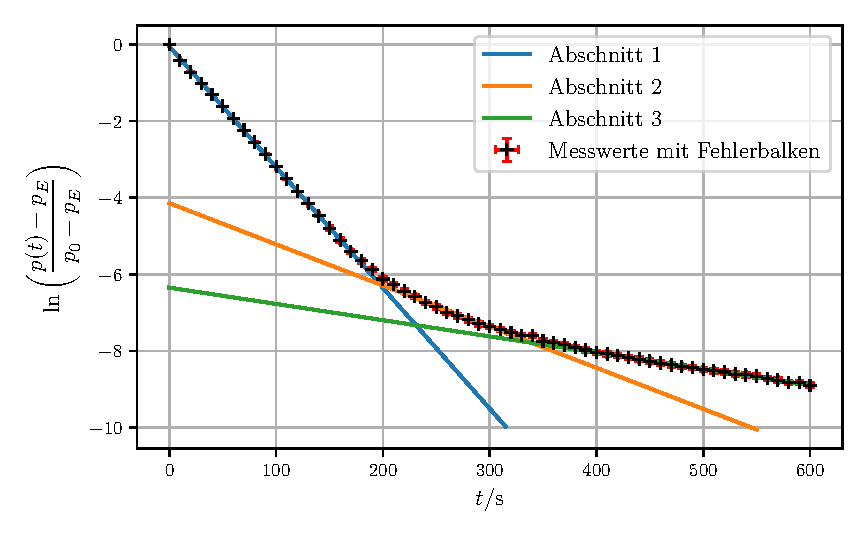
\includegraphics[width=0.8\textwidth]{abb/dreh_evac.pdf}
        \caption{Die logarithmische Evakuierungskurve der Drehschieberpumpe.}
        \label{fig:drehEvac}
    \end{figure}

    \begin{longtable}{S[table-format=3.1(1)] S[table-format=3.3(3)] S[table-format=3.3(3)] S[table-format=3.3(3)]}
        \centering\\
        \label{tab:drehEvac}\\
        \caption{Messergebnisse der Evakuierungskurve zur Drehschieberpumpe.}\\
        \toprule
        {$t/\si{\second}$} & {$p_1/\si{\milli\bar}$} & {$p_2/\si{\milli\bar}$} & {$p_3/\si{\milli\bar}$} \\
        \midrule
        \endfirsthead
        \caption{Messergebnisse der Evakuierungskurve zur Drehschieberpumpe.}\\
        \toprule
        {$t/\si{\second}$} & {$p_1/\si{\milli\bar}$} & {$p_2/\si{\milli\bar}$} & {$p_3/\si{\milli\bar}$} \\
        \midrule
        \endhead
        \bottomrule
        \endfoot
        \bottomrule
        \endlastfoot
        10.0(2) & 660.9(2.0) & 646.3(1.9) & 659.0(2.0)\\ 
        20.0(2) & 488.1(1.5) & 498.3(1.5) & 474.6(1.4)\\ 
        30.0(2) & 364.7(1.1) & 360.3(1.1) & 364.0(1.1)\\ 
        40.0(2) & 271.50(81) & 268.60(81) & 271.60(81)\\ 
        50.0(2) & 199.60(60) & 198.40(60) & 201.90(61)\\ 
        60.0(2) & 145.10(44) & 144.20(43) & 146.80(44)\\ 
        70.0(2) & 106.20(32) & 106.00(32) & 107.60(32)\\ 
        80.0(2) & 79.30(24) & 77.10(23) & 78.10(23)\\ 
        90.0(2) & 58.10(17) & 56.30(17) & 57.00(17)\\ 
        100.0(2) & 41.90(13) & 40.90(12) & 41.60(12)\\ 
        110.0(2) & 30.20(9) & 29.60(9) & 29.90(9)\\ 
        120.0(2) & 21.80(7) & 21.50(7) & 21.90(7)\\ 
        130.0(2) & 16.00(5) & 15.50(5) & 15.90(5)\\ 
        140.0(2) & 11.30(3) & 11.30(3) & 11.60(4)\\ 
        150.0(2) & 8.30(83) & 8.20(82) & 8.30(83)\\ 
        160.0(2) & 6.10(61) & 6.00(60) & 6.10(61)\\ 
        170.0(2) & 4.50(45) & 4.50(45) & 4.50(45)\\ 
        180.0(2) & 3.60(36) & 3.50(35) & 3.50(35)\\ 
        190.0(2) & 2.90(29) & 2.80(28) & 2.80(28)\\ 
        200.0(2) & 2.20(22) & 2.20(22) & 2.20(22)\\ 
        210.0(2) & 1.90(19) & 1.90(19) & 1.90(19)\\ 
        220.0(2) & 1.60(16) & 1.60(16) & 1.60(16)\\ 
        230.0(2) & 1.40(14) & 1.40(14) & 1.40(14)\\ 
        240.0(2) & 1.20(12) & 1.20(12) & 1.20(12)\\ 
        250.0(2) & 1.00(10) & 1.10(11) & 1.10(11)\\ 
        260.0(2) & 0.900(90) & 0.930(93) & 0.940(94)\\ 
        270.0(2) & 0.840(84) & 0.840(84) & 0.850(85)\\ 
        280.0(2) & 0.760(76) & 0.770(77) & 0.760(76)\\ 
        290.0(2) & 0.680(68) & 0.690(69) & 0.690(69)\\ 
        300.0(2) & 0.640(64) & 0.640(64) & 0.640(64)\\ 
        310.0(2) & 0.600(60) & 0.590(59) & 0.590(59)\\ 
        320.0(2) & 0.550(55) & 0.550(55) & 0.550(55)\\ 
        330.0(2) & 0.500(50) & 0.510(51) & 0.510(51)\\ 
        340.0(2) & 0.570(57) & 0.470(47) & 0.480(48)\\ 
        350.0(2) & 0.440(44) & 0.440(44) & 0.440(44)\\ 
        360.0(2) & 0.420(42) & 0.420(42) & 0.420(42)\\ 
        370.0(2) & 0.400(40) & 0.390(39) & 0.410(41)\\ 
        380.0(2) & 0.370(37) & 0.380(38) & 0.370(37)\\ 
        390.0(2) & 0.350(35) & 0.350(35) & 0.350(35)\\ 
        400.0(2) & 0.330(33) & 0.330(33) & 0.330(33)\\ 
        410.0(2) & 0.320(32) & 0.310(31) & 0.320(32)\\ 
        420.0(2) & 0.310(31) & 0.300(30) & 0.300(30)\\ 
        430.0(2) & 0.290(29) & 0.290(29) & 0.290(29)\\ 
        440.0(2) & 0.280(28) & 0.280(28) & 0.270(27)\\ 
        450.0(2) & 0.270(27) & 0.260(26) & 0.260(26)\\ 
        460.0(2) & 0.250(25) & 0.250(25) & 0.250(25)\\ 
        470.0(2) & 0.240(24) & 0.240(24) & 0.240(24)\\ 
        480.0(2) & 0.230(23) & 0.230(23) & 0.230(23)\\ 
        490.0(2) & 0.230(23) & 0.220(22) & 0.220(22)\\ 
        500.0(2) & 0.220(22) & 0.210(21) & 0.210(21)\\ 
        510.0(2) & 0.210(21) & 0.200(20) & 0.210(21)\\ 
        520.0(2) & 0.200(20) & 0.200(20) & 0.200(20)\\ 
        530.0(2) & 0.190(19) & 0.190(19) & 0.190(19)\\ 
        540.0(2) & 0.190(19) & 0.190(19) & 0.180(18)\\ 
        550.0(2) & 0.180(18) & 0.180(18) & 0.180(18)\\ 
        560.0(2) & 0.170(17) & 0.170(17) & 0.170(17)\\ 
        570.0(2) & 0.160(16) & 0.170(17) & 0.160(16)\\ 
        580.0(2) & 0.150(15) & 0.160(16) & 0.150(15)\\ 
        590.0(2) & 0.150(15) & 0.160(16) & 0.150(15)\\ 
        600.0(2) & 0.140(14) & 0.150(15) & 0.140(14)     
    \end{longtable}

    \begin{longtable}{S[table-format=3.1(1)] S[table-format=3.4(4)] S[table-format=3.4(4)]}
        \centering\\
        \label{tab:drehEvacMean}\\
        \caption{Mittelwert und logarithmischer Ausdruck der Evakuierungskurve der Drehschieberpumpe.}\\
        {$t/\si{\second}$} & {$p/\si{\milli\bar}$} & {$\ln\left(\frac{p-p_E}{p_0-p_E}\right)$} \\
        \hline
        \endfirsthead
        \caption{Mittelwert und logarithmischer Ausdruck der Evakuierungskurve der Drehschieberpumpe.}\\
        {$t/\si{\second}$} & {$p/\si{\milli\bar}$} & {$\ln\left(\frac{p-p_E}{p_0-p_E}\right)$} \\
        \hline
        \endhead
        \hline
        \endfoot
        \hline
        \endlastfoot 
        10.0(2) & 655.4(1.1) & -0.4225(24) \\ 
        20.0(2) & 487.00(84) & -0.7195(24) \\ 
        30.0(2) & 363.00(63) & -1.0134(24) \\ 
        40.0(2) & 270.57(47) & -1.3073(24) \\ 
        50.0(2) & 199.97(35) & -1.6096(24) \\ 
        60.0(2) & 145.37(25) & -1.9285(24) \\ 
        70.0(2) & 106.60(18) & -2.2387(24) \\ 
        80.0(2) & 78.17(14) & -2.5490(24) \\ 
        90.0(2) & 57.133(99) & -2.8625(24) \\ 
        100.0(2) & 41.467(72) & -3.1830(24) \\ 
        110.0(2) & 29.900(52) & -3.5101(24) \\ 
        120.0(2) & 21.733(38) & -3.8292(25) \\ 
        130.0(2) & 15.800(27) & -4.1482(25) \\ 
        140.0(2) & 11.400(20) & -4.4747(25) \\ 
        150.0(2) & 8.27(48) & -4.80(6) \\ 
        160.0(2) & 6.07(35) & -5.11(6) \\ 
        170.0(2) & 4.50(26) & -5.41(6) \\ 
        180.0(2) & 3.53(20) & -5.65(6) \\ 
        190.0(2) & 2.83(16) & -5.87(6) \\ 
        200.0(2) & 2.20(13) & -6.12(6) \\ 
        210.0(2) & 1.90(11) & -6.27(6) \\ 
        220.0(2) & 1.600(92) & -6.44(6) \\ 
        230.0(2) & 1.400(81) & -6.58(6) \\ 
        240.0(2) & 1.200(69) & -6.73(6) \\ 
        250.0(2) & 1.067(62) & -6.85(6) \\ 
        260.0(2) & 0.923(53) & -6.99(6) \\ 
        270.0(2) & 0.843(49) & -7.09(6) \\ 
        280.0(2) & 0.763(44) & -7.19(6) \\ 
        290.0(2) & 0.687(40) & -7.29(6) \\ 
        300.0(2) & 0.640(37) & -7.36(6) \\ 
        310.0(2) & 0.593(34) & -7.44(6) \\ 
        320.0(2) & 0.550(32) & -7.52(6) \\ 
        330.0(2) & 0.507(29) & -7.60(6) \\ 
        340.0(2) & 0.507(29) & -7.60(6) \\ 
        350.0(2) & 0.440(25) & -7.74(6) \\ 
        360.0(2) & 0.420(24) & -7.79(6) \\ 
        370.0(2) & 0.400(23) & -7.84(6) \\ 
        380.0(2) & 0.373(22) & -7.91(6) \\ 
        390.0(2) & 0.350(20) & -7.98(6) \\ 
        400.0(2) & 0.330(19) & -8.04(6) \\ 
        410.0(2) & 0.317(18) & -8.08(6) \\ 
        420.0(2) & 0.303(18) & -8.12(6) \\ 
        430.0(2) & 0.290(17) & -8.17(6) \\ 
        440.0(2) & 0.277(16) & -8.22(6) \\ 
        450.0(2) & 0.263(15) & -8.27(6) \\ 
        460.0(2) & 0.250(14) & -8.32(6) \\ 
        470.0(2) & 0.240(14) & -8.36(6) \\ 
        480.0(2) & 0.230(13) & -8.41(6) \\ 
        490.0(2) & 0.223(13) & -8.44(6) \\ 
        500.0(2) & 0.213(12) & -8.48(6) \\ 
        510.0(2) & 0.207(12) & -8.52(6) \\ 
        520.0(2) & 0.200(12) & -8.55(6) \\ 
        530.0(2) & 0.190(11) & -8.60(6) \\ 
        540.0(2) & 0.187(11) & -8.62(6) \\ 
        550.0(2) & 0.180(10) & -8.66(6) \\ 
        560.0(2) & 0.1700(98) & -8.72(6) \\ 
        570.0(2) & 0.1633(94) & -8.76(6) \\ 
        580.0(2) & 0.1533(89) & -8.83(6) \\ 
        590.0(2) & 0.1533(89) & -8.83(6) \\ 
        600.0(2) & 0.1433(83) & -8.90(6) \\      
    \end{longtable}

    \subsubsection{Leckratenmessung}
    Die Messung wurde mit den Gleichgewichtsdrücken $p_g$ = 0.5; 10; 50; und 100 \unit{\milli\bar} durchgeführt.
    Die zugehörigen Messergebnisse sind in Tabellen \ref{tab:drehLeckRaw05}, \ref{tab:drehLeckRaw10}, \ref{tab:drehLeckRaw50} und \ref{tab:drehLeckRaw100}
    gelistet. Dabei wurde der Fehler des Mittelwertes
    nach \autoref{eq:fehlerDesMittelwertes} berechnet.\\

    Der lineare Ausgleichsparameter $a$ aus
    \begin{equation*}
        p(t) = a\cdot t + b
    \end{equation*}
    wird benötigt um als Steigung $\frac{\text{d}p}{\text{d}p}$ der $p(t)$ Kurve in \autoref{eq:leckSaug} einzusetzen.
    Die erhaltenen Parameter und die daraus resultierenden Saugvermögen sind in Abhängigkeit der anfänglichen Gleichgewichtsdrücke in \autoref{tab:drehLeckSaug} aufgeführt. Mit 
    \begin{equation*}
        \sigma_Q = \sqrt{(a\cdot\sigma_{V_0})^2 + (V_0 \cdot \sigma_a)^2}
    \end{equation*}
    lässt sich der Fehler des Saugvermögens
    \begin{equation}
        \sigma_S = \sqrt{\left(\frac{\sigma_Q}{p_g}\right)^2 + (Q\cdot\sigma_{p_g})^2} = \sqrt{\frac{1}{p_g^2}\left[(a\cdot\sigma_{V_0})^2 + (V_0 \cdot \sigma_a)^2\right] + (Q\cdot\sigma_{p_g})^2}
        \label{eq:errS}
    \end{equation}
    berechnen.
    
    In Abbildungen \ref{fig:drehLeck05}, \ref{fig:drehLeck10}, \ref{fig:drehLeck50} und \ref{fig:drehLeck100} sind die $p(t)$-Kurven samt ihrer Ausgleichsgeraden graphisch dargstellt.
    \begin{table}
        \centering
        \caption{Ausgleichsparameter und Saugvermögen der Leckratenmessung zur Drehschieberpumpe.}
        \label{tab:drehLeckSaug}
        \begin{tabular}{c|S[table-format=1.5(5)] S[table-format=3.3(3)] S[table-format=1.2(2)]}
            \toprule
            {$p_g/\unit{\milli\bar}$} & {$a/\unit{\milli\bar\per\second}$} & {$b/\unit{\milli\bar}$} & {$S/\unit{\liter\per\second}$} \\
            \midrule
            0.5 & 0.00907(10) & 1.637(11) & 0.62(7)\\
            10& 0.38500(28) & 15.967(34) & 1.31(13)\\
            50& 1.7246(16) & 58.30(20) & 1.17(12)\\
            100& 3.223(22) & 120.4(2.7) & 1.10(11)\\
            \bottomrule
        \end{tabular}
    \end{table}

    \begin{table}
        \centering
        \caption{Messergebnisse der Leckratenmessung zur Drehschieberpumpe für $p_g=\qty{0.5}{\milli\bar}$.}
        \label{tab:drehLeckRaw05}
        \sisetup{table-format=1.2(2)}
        \begin{tabular}{S[table-format=3.1(1)]SSSS}
            \toprule
            & \multicolumn{3}{c}{$p_g = \qty{0.5}{\milli\bar}$} & {Mittelwert}\\
            \cmidrule(lr){2-4}\cmidrule(lr){5-5}
            {$t/\unit{\second}$} & {$p_1/\unit{\milli\bar}$} & {$p_2/\unit{\milli\bar}$} & {$p_3/\unit{\milli\bar}$} & {$p/\unit{\milli\bar}$}\\
            \midrule
            10.0(2) & 1.70(17) & 1.70(17) & 1.70(17) & 1.70(10)\\ 
            20.0(2) & 1.80(18) & 1.80(18) & 1.80(18) & 1.80(10)\\ 
            30.0(2) & 1.90(19) & 1.90(19) & 1.90(19) & 1.90(11)\\ 
            40.0(2) & 2.00(20) & 2.00(20) & 2.00(20) & 2.00(12)\\ 
            50.0(2) & 2.10(21) & 2.10(21) & 2.10(21) & 2.10(12)\\ 
            60.0(2) & 2.10(21) & 2.20(22) & 2.20(22) & 2.17(13)\\ 
            70.0(2) & 2.20(22) & 2.30(23) & 2.30(23) & 2.27(13)\\ 
            80.0(2) & 2.30(23) & 2.40(24) & 2.40(24) & 2.37(14)\\ 
            90.0(2) & 2.40(24) & 2.50(25) & 2.50(25) & 2.47(14)\\ 
            100.0(2) & 2.50(25) & 2.60(26) & 2.60(26) & 2.57(15)\\ 
            110.0(2) & 2.60(26) & 2.70(27) & 2.70(27) & 2.67(15)\\ 
            120.0(2) & 2.70(27) & 2.80(28) & 2.80(28) & 2.77(16)\\ 
            130.0(2) & 2.80(28) & 2.90(29) & 2.90(29) & 2.87(17)\\ 
            140.0(2) & 2.90(29) & 3.00(30) & 2.90(29) & 2.93(17)\\ 
            150.0(2) & 2.90(29) & 3.00(30) & 3.00(30) & 2.97(17)\\ 
            160.0(2) & 3.00(30) & 3.10(31) & 3.10(31) & 3.07(18)\\ 
            170.0(2) & 3.10(31) & 3.20(32) & 3.20(32) & 3.17(18)\\ 
            180.0(2) & 3.20(32) & 3.30(33) & 3.30(33) & 3.27(19)\\ 
            190.0(2) & 3.20(32) & 3.40(34) & 3.40(34) & 3.33(19)\\ 
            200.0(2) & 3.30(33) & 3.50(35) & 3.50(35) & 3.43(20)\\  
            \bottomrule
        \end{tabular}
    \end{table}

    \begin{table}
        \centering
        \caption{Messergebnisse der Leckratenmessung zur Drehschieberpumpe für $p_g = \qty{10}{\milli\bar}$.}
        \label{tab:drehLeckRaw10}
        \sisetup{table-format=2.2(2)}
        \begin{tabular}{S[table-format=3.1(1)]SSSS}
            \toprule
            & \multicolumn{3}{c}{$p_g = \qty{10}{\milli\bar}$} & {Mittelwert}\\
            \cmidrule(lr){2-4}\cmidrule(lr){5-5}
            {$t/\unit{\second}$} & {$p_1/\unit{\milli\bar}$} & {$p_2/\unit{\milli\bar}$} & {$p_3/\unit{\milli\bar}$} & {$p/\unit{\milli\bar}$}\\
            \midrule
            10.0(2) & 19.30(6) & 20.00(6) & 19.80(6) & 19.70(3)\\ 
            20.0(2) & 23.20(7) & 23.90(7) & 23.80(7) & 23.63(4)\\ 
            30.0(2) & 27.10(8) & 27.70(8) & 27.60(8) & 27.47(5)\\ 
            40.0(2) & 30.90(9) & 31.60(9) & 31.50(9) & 31.33(5)\\ 
            50.0(2) & 35.10(11) & 35.40(11) & 35.30(11) & 35.27(6)\\ 
            60.0(2) & 38.90(12) & 39.40(12) & 39.20(12) & 39.17(7)\\ 
            70.0(2) & 42.90(13) & 43.10(13) & 43.00(13) & 43.00(7)\\ 
            80.0(2) & 46.60(14) & 47.10(14) & 46.90(14) & 46.87(8)\\ 
            90.0(2) & 50.10(15) & 50.80(15) & 50.60(15) & 50.50(9)\\ 
            100.0(2) & 54.30(16) & 54.70(16) & 54.60(16) & 54.53(9)\\ 
            110.0(2) & 58.20(17) & 58.50(18) & 58.30(17) & 58.33(10)\\ 
            120.0(2) & 61.70(19) & 62.40(19) & 62.20(19) & 62.10(11)\\ 
            130.0(2) & 65.80(20) & 66.20(20) & 66.10(20) & 66.03(11)\\ 
            140.0(2) & 69.70(21) & 70.10(21) & 70.00(21) & 69.93(12)\\ 
            150.0(2) & 73.50(22) & 74.00(22) & 73.80(22) & 73.77(13)\\ 
            160.0(2) & 77.40(23) & 77.70(23) & 77.60(23) & 77.57(13)\\ 
            170.0(2) & 81.20(24) & 81.60(24) & 81.50(24) & 81.43(14)\\ 
            180.0(2) & 84.70(25) & 85.50(26) & 85.70(26) & 85.30(15)\\ 
            190.0(2) & 88.90(27) & 89.00(27) & 89.10(27) & 89.00(15)\\ 
            200.0(2) & 92.70(28) & 93.10(28) & 92.90(28) & 92.90(16)\\   
            \bottomrule
        \end{tabular}
    \end{table}

    \begin{table}
        \centering
        \caption{Messergebnisse der Leckratenmessung zur Drehschieberpumpe für $p_g=\qty{50}{\milli\bar}$.}
        \label{tab:drehLeckRaw50}
        \sisetup{table-format=3.2(2)}
        \begin{tabular}{S[table-format=3.1(1)]SSSS}
            \toprule
            & \multicolumn{3}{c}{$p_g = \qty{50}{\milli\bar}$} & {Mittelwert}\\
            \cmidrule(lr){2-4}\cmidrule(lr){5-5}
            {$t/\unit{\second}$} & {$p_1/\unit{\milli\bar}$} & {$p_2/\unit{\milli\bar}$} & {$p_3/\unit{\milli\bar}$} & {$p/\unit{\milli\bar}$}\\
            \midrule 
            10.0(2) & 74.20(22) & 75.50(23) & 76.10(23) & 75.27(13)\\ 
            20.0(2) & 91.20(27) & 93.10(28) & 93.40(28) & 92.57(16)\\ 
            30.0(2) & 108.20(32) & 110.40(33) & 110.90(33) & 109.83(19)\\ 
            40.0(2) & 125.1(4) & 127.8(4) & 128.2(4) & 127.03(22)\\ 
            50.0(2) & 142.0(4) & 145.1(4) & 145.5(4) & 144.20(25)\\ 
            60.0(2) & 159.0(5) & 162.6(5) & 162.9(5) & 161.50(28)\\ 
            70.0(2) & 176.3(5) & 181.5(5) & 180.2(5) & 179.33(31)\\ 
            80.0(2) & 194.5(6) & 197.1(6) & 197.5(6) & 196.37(34)\\ 
            90.0(2) & 208.9(6) & 215.3(6) & 218.7(7) & 214.3(4)\\ 
            100.0(2) & 227.6(7) & 232.4(7) & 233.2(7) & 231.1(4)\\ 
            110.0(2) & 244.5(7) & 250.0(8) & 250.6(8) & 248.4(4)\\ 
            120.0(2) & 261.5(8) & 267.4(8) & 267.9(8) & 265.6(5)\\ 
            130.0(2) & 280.0(8) & 284.8(9) & 285.2(9) & 283.3(5)\\ 
            140.0(2) & 293.4(9) & 302.2(9) & 302.5(9) & 299.4(5)\\ 
            150.0(2) & 310.6(9) & 319.4(1.0) & 319.8(1.0) & 316.6(5)\\ 
            160.0(2) & 329.2(1.0) & 336.8(1.0) & 337.4(1.0) & 334.5(6)\\ 
            170.0(2) & 346.2(1.0) & 354.2(1.1) & 354.7(1.1) & 351.7(6)\\ 
            180.0(2) & 363.0(1.1) & 371.5(1.1) & 370.1(1.1) & 368.2(6)\\ 
            190.0(2) & 379.9(1.1) & 388.8(1.2) & 387.5(1.2) & 385.4(7)\\ 
            200.0(2) & 396.7(1.2) & 405.9(1.2) & 406.5(1.2) & 403.0(7)\\ 
        \bottomrule
        \end{tabular}
    \end{table}

    \begin{table}
        \centering
        \caption{Messergebnisse der Leckratenmessung zur Drehschieberpumpe für $p_g=\qty{100}{\milli\bar}$.}
        \label{tab:drehLeckRaw100}
        \sisetup{table-format=3.1(1)}
        \begin{tabular}{SSSSS}
            \toprule
            & \multicolumn{3}{c}{$p_g = \qty{100}{\milli\bar}$} & {Mittelwert}\\
            \cmidrule(lr){2-4}\cmidrule(lr){5-5}
            {$t/\unit{\second}$} & {$p_1/\unit{\milli\bar}$} & {$p_2/\unit{\milli\bar}$} & {$p_3/\unit{\milli\bar}$} & {$p/\unit{\milli\bar}$}\\
            \midrule 
            10.0(2) & 145.8(4) & 147.1(4) & 146.3(4) & 146.4(3)\\ 
            20.0(2) & 179.6(5) & 177.6(5) & 180.2(5) & 179.1(3)\\ 
            30.0(2) & 212.0(6) & 213.4(6) & 212.5(6) & 212.6(4)\\ 
            40.0(2) & 245.7(7) & 247.1(7) & 246.4(7) & 246.4(4)\\ 
            50.0(2) & 279.5(8) & 280.0(8) & 280.1(8) & 279.9(5)\\ 
            60.0(2) & 313.2(9) & 314.6(9) & 313.9(9) & 313.9(5)\\ 
            70.0(2) & 347.0(1.0) & 351.7(1.1) & 347.5(1.0) & 348.7(6)\\ 
            80.0(2) & 380.5(1.1) & 382.0(1.1) & 381.1(1.1) & 381.2(7)\\ 
            90.0(2) & 414.0(1.2) & 415.4(1.2) & 414.6(1.2) & 414.7(7)\\ 
            100.0(2) & 447.3(1.3) & 448.5(1.3) & 447.8(1.3) & 447.9(8)\\ 
            110.0(2) & 480.3(1.4) & 481.4(1.4) & 484.0(1.5) & 481.9(8)\\ 
            120.0(2) & 513.0(1.5) & 514.0(1.5) & 513.4(1.5) & 513.5(9)\\ 
            130.0(2) & 545.0(1.6) & 546.0(1.6) & 545.5(1.6) & 545.5(9)\\ 
            140.0(2) & 576.4(1.7) & 578.0(1.7) & 577.0(1.7) & 577.1(1.0)\\ 
            150.0(2) & 607.8(1.8) & 608.9(1.8) & 608.1(1.8) & 608.3(1.1)\\ 
            160.0(2) & 638.3(1.9) & 639.2(1.9) & 638.5(1.9) & 638.7(1.1)\\ 
            170.0(2) & 667.9(2.0) & 668.9(2.0) & 668.3(2.0) & 668.4(1.2)\\ 
            180.0(2) & 696.5(2.1) & 697.0(2.1) & 697.0(2.1) & 696.8(1.2)\\ 
            190.0(2) & 724.6(2.2) & 725.3(2.2) & 724.7(2.2) & 724.9(1.3)\\ 
            200.0(2) & 751.2(2.3) & 752.1(2.3) & 751.5(2.3) & 751.6(1.3)\\ 
            \bottomrule
        \end{tabular}
    \end{table}

    \begin{figure}
        \centering
        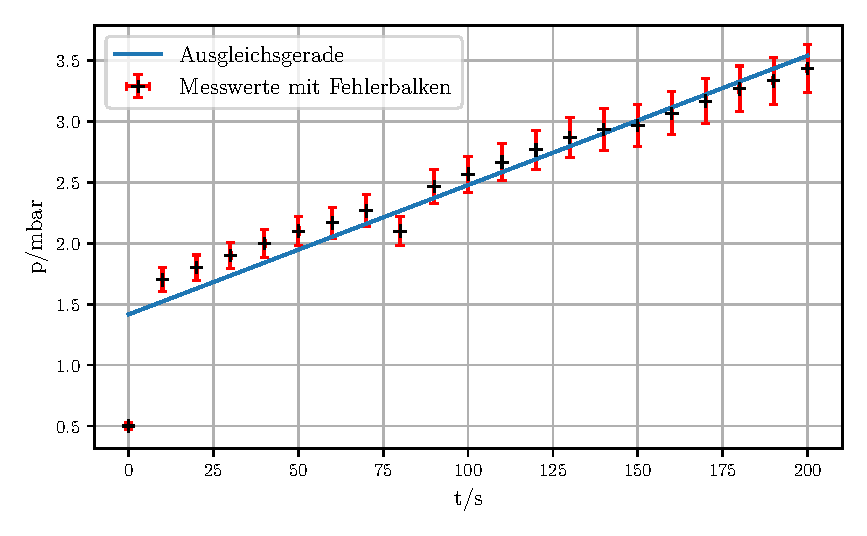
\includegraphics[width=0.8\textwidth]{abb/dreh_leck0.5.pdf}
        \caption{Messergebnisse und Ausgleichsgeraden der Leckratenmessung zur Drehschieberpumpe mit $p_g = \qty{0.5}{\milli\bar}$.}
        \label{fig:drehLeck05}
    \end{figure}

    \begin{figure}
        \centering
        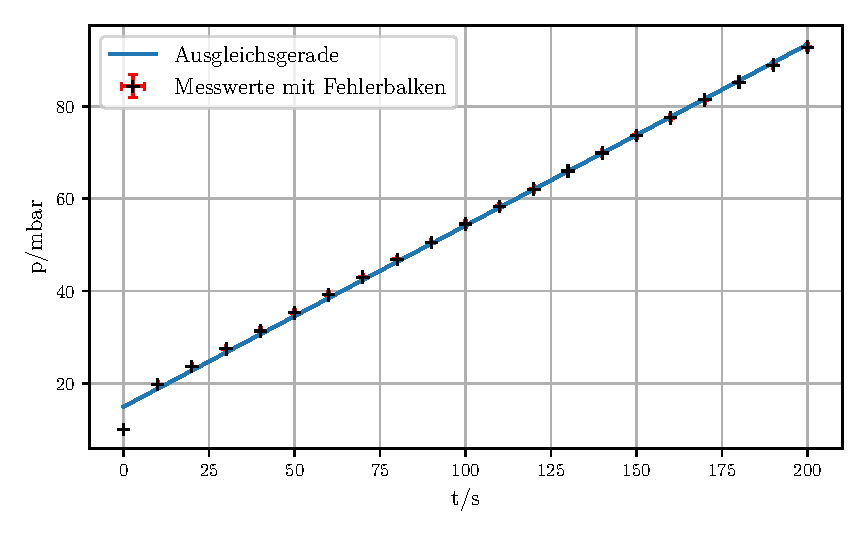
\includegraphics[width=0.8\textwidth]{abb/dreh_leck10.pdf}
        \caption{Messergebnisse und Ausgleichsgeraden der Leckratenmessung zur Drehschieberpumpe mit $p_g = \qty{10}{\milli\bar}$.}
        \label{fig:drehLeck10}
    \end{figure}

    \begin{figure}
        \centering
        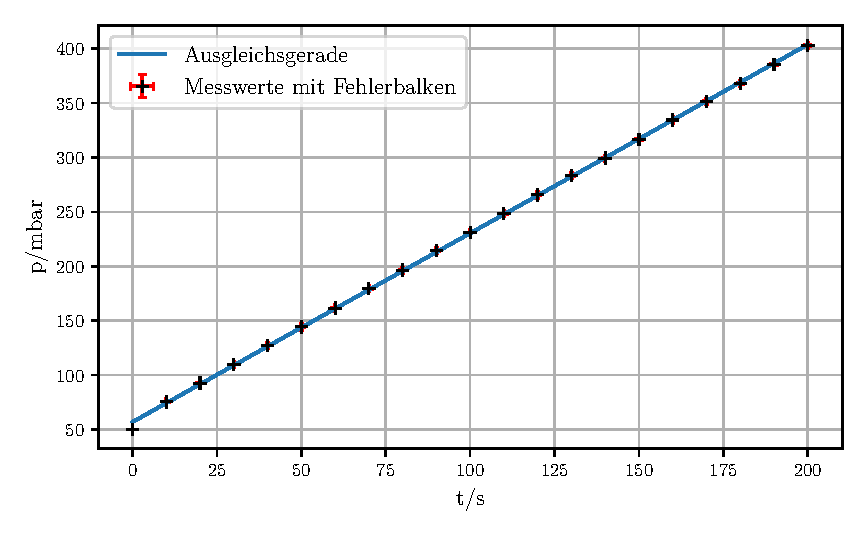
\includegraphics[width=0.8\textwidth]{abb/dreh_leck50.pdf}
        \caption{Messergebnisse und Ausgleichsgeraden der Leckratenmessung zur Drehschieberpumpe mit $p_g = \qty{50}{\milli\bar}$.}
        \label{fig:drehLeck50}
    \end{figure}

    \begin{figure}
        \centering
        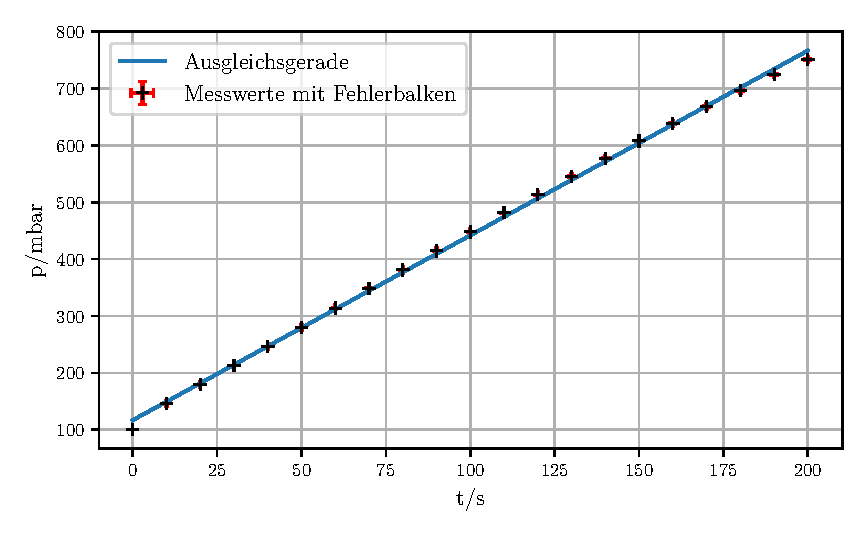
\includegraphics[width=0.8\textwidth]{abb/dreh_leck100.pdf}
        \caption{Messergebnisse und Ausgleichsgeraden der Leckratenmessung zur Drehschieberpumpe mit $p_g = \qty{100}{\milli\bar}$.}
        \label{fig:drehLeck100}
    \end{figure}
    
\newpage
\subsection{Turbomolekularpumpe}
    Zur Auswertung wurde das Rezipientenvolumen $V_0 = \SI{33(3.3)}{\liter}$\cite{sample}, der Enddruck $p_E = \qty{1.4(4)e-5}{\milli\bar}$
    und der Startdruck $p_0 = \qty{5(1.5)e-3}{\milli\bar}$ benutzt.

    \subsubsection{Evakuierungskurve}

    In \autoref{tab:turboEvac} sind die Messergebnisse aufgelistet. Der Mittelwert $p$ dieser Messreihe und der logarithmische Ausdruck
    $\ln\left(\frac{p-p_E}{p_0-p_E}\right)$, dessen Fehler sich analog zu \autoref{eq:ln} berechnen lässt
    Durch eine lineare Ausgleichsrechnung 
    \begin{equation*}
        \ln\left(\frac{p-p_E}{p_0-p_E}\right) = a_i \cdot t + b_i
    \end{equation*}
    an die drei Abschnitte des Ausdrucks ergeben sich folgende Parameter:
    \begin{align*}
        a_1 &= \qty{-0.35038}{\per\second} & b_1 &= \num{-1.57} \\
        a_2 &= \qty{-0.11626}{\per\second} & b_2 &= \num{-2.341} \\
        a_3 &= \qty{-0.00439(29)}{\per\second} & b_3 &= \num{-4.837(23)}
    \end{align*}
    Hierbei enthalten die Paramter für den ersten und zweiten Abschnitt keine Abweichungen, da jeweils lediglich zwei Messwerte benutzt werden können und eine direkte
    Verbindung dieser Beiden Steigung und Startwert der Ausgleichsgerade festlegt. Es bräuchte mindestens einen weiteren Messwert um durch die lineare Regression eine Kovarianz zu erhalten.
    Die zugehörigen Ausgleichsgeraden sind in \autoref{fig:turboEvac} eingezeichnet. Aufgrund der logarithmischen Skala ist zu Beginn der Messung nur schwer ein Messfehler zu erkennen,
    da er ausreichend klein ist, um in der graphischen Darstellung fast gänzlich hinter der Markierung des Messwertes zu verschwinden.

    Nach Umstellen von \autoref{eq:evacSaug} und mit Einsetzen von $a_i$ für $\frac{dp}{dt}$
    lässt sich das Saugvermögen abschnittsweise berechnen zu:
    \begin{align*}
        S_1 &= \qty{11.56(1.16)}{\liter\per\second} \\
        S_2 &= \qty{3.84(38)}{\liter\per\second} \\
        S_3 &= \qty{0.14(1)}{\liter\per\second} 
    \end{align*}

    \begin{figure}
        \centering
        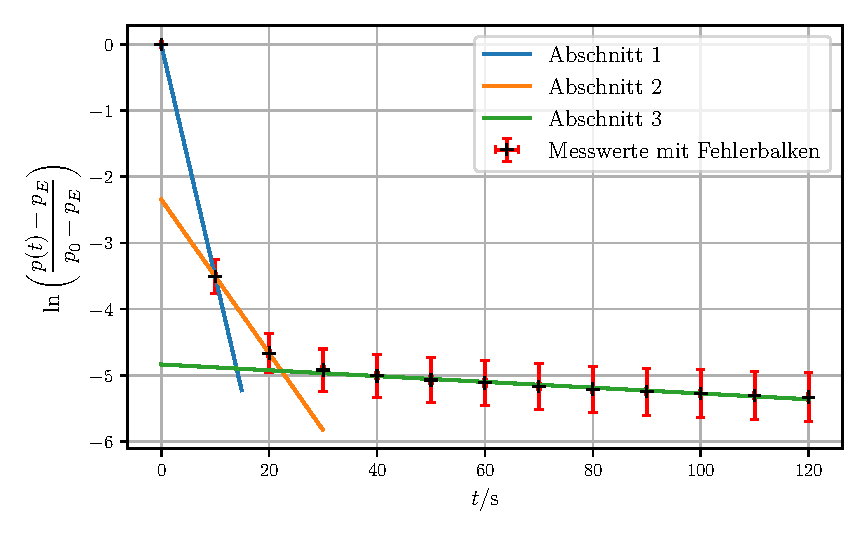
\includegraphics[width=0.8\textwidth]{abb/turbo_evac.pdf}
        \caption{Die logarithmische Evakuierungskurve der Turbomolekularpumpe.}
        \label{fig:turboEvac}
    \end{figure}

    \begin{table}
        \centering
        \caption{Messergebnisse der Evakuierungskurve zur Turbomolekularpumpe.}
        \label{tab:turboEvac}
        \sisetup{table-format=1.2(2)e-04}
        \begin{tabular}{S[table-format=3.1(1)]SSS}
            \toprule
            {$t/\si{\second}$} & {$p_1/\si{\milli\bar}$} & {$p_2/\si{\milli\bar}$} & {$p_3/\si{\milli\bar}$} \\
            \midrule 
            10.0(2) & 1.6(0.48)e-04 & 1.67(50)e-04 & 1.65(49)e-04 \\ 
            20.0(2) & 6.2(1.9)e-05 & 6.0(1.8)e-05 & 6.0(1.8)e-05 \\ 
            30.0(2) & 5.1(1.5)e-05 & 5.1(1.5)e-05 & 4.9(1.5)e-05 \\ 
            40.0(2) & 4.8(1.4)e-05 & 4.7(1.4)e-05 & 4.7(1.4)e-05 \\ 
            50.0(2) & 4.5(1.4)e-05 & 4.6(1.4)e-05 & 4.4(1.3)e-05 \\ 
            60.0(2) & 4.6(1.4)e-05 & 4.4(1.3)e-05 & 4.2(1.3)e-05 \\ 
            70.0(2) & 4.4(1.3)e-05 & 4.2(1.3)e-05 & 4.0(1.2)e-05 \\ 
            80.0(2) & 4.3(1.3)e-05 & 4.1(1.2)e-05 & 3.9(1.2)e-05 \\ 
            90.0(2) & 4.2(1.3)e-05 & 4.0(1.2)e-05 & 3.8(1.2)e-05 \\ 
            100.0(2) & 4.1(1.2)e-05 & 3.9(1.2)e-05 & 3.8(1.1)e-05 \\ 
            110.0(2) & 4.0(1.2)e-05 & 3.9(1.2)e-05 & 3.7(1.1)e-05 \\ 
            120.0(2) & 4.0(1.2)e-05 & 3.8(1.1)e-05 & 3.6(1.1)e-05 \\
            \bottomrule
        \end{tabular}
    \end{table}

    \begin{table}
        \centering
        \caption{Messergebnisse der Evakuierungskurve zur Turbomolekularpumpe.}
        \label{tab:turboEvacMean}
        \begin{tabular}{S[table-format=3.1(1)]S[table-format=1.2(2)e-04]S[table-format=3.2(2)]}
            \toprule
            {$t/\si{\second}$} & {$p/\si{\milli\bar}$} & {$\ln\left(\frac{p-p_E}{p_0-p_E}\right)$} \\
            \midrule 
            10.0(2) & 1.64(28)e-04 & -3.50(26) \\ 
            20.0(2) & 6.1(1.1)e-05 & -4.67(30) \\ 
            30.0(2) & 5.04(87)e-05 & -4.92(32) \\ 
            40.0(2) & 4.73(82)e-05 & -5.01(33) \\ 
            50.0(2) & 4.53(79)e-05 & -5.07(33) \\ 
            60.0(2) & 4.39(76)e-05 & -5.12(34) \\ 
            70.0(2) & 4.23(73)e-05 & -5.17(34) \\ 
            80.0(2) & 4.12(71)e-05 & -5.21(35) \\ 
            90.0(2) & 4.02(70)e-05 & -5.2(4) \\ 
            100.0(2) & 3.95(68)e-05 & -5.3(4) \\ 
            110.0(2) & 3.87(67)e-05 & -5.3(4) \\ 
            120.0(2) & 3.81(66)e-05 & -5.3(4) \\
            \bottomrule
        \end{tabular}
    \end{table}

    \newpage
    \subsubsection{Leckratenmessung}
    Die Messung wurde mit den Gleichgewichtsdrücken $p_g = \num{2e-4}$; $\num{1e-4}$; $\num{7e-5}$; und $\qty{5e-5}{\milli\bar}$ durchgeführt.
    Die zugehörigen Messergebnisse sind in Tabellen \ref{tab:turboLeckRaw2}, \ref{tab:turboLeckRaw1}, \ref{tab:turboLeckRaw7} und \ref{tab:turboLeckRaw5}
    gelistet. Dabei wurde der Fehler des Mittelwertes
    nach \autoref{eq:fehlerDesMittelwertes} berechnet.\\

    Der lineare Ausgleichsparameter $a$ aus
    \begin{equation*}
        p(t) = a\cdot t + b
    \end{equation*}
    wird benötigt um als Steigung $\frac{\text{d}p}{\text{d}p}$ der $p(t)$ Kurve in \autoref{eq:leckSaug} einzusetzen.
    Die erhaltenen Parameter und die daraus resultierenden Saugvermögen sind in Abhängigkeit der anfänglichen Gleichgewichtsdrücke in \autoref{tab:turboLeckSaug} aufgeführt.
    Dabei wird der Fehler des Saugvermögens analog zu \autoref{eq:errS} berechnet.
    In Abbildungen \ref{fig:turboLeck2}, \ref{fig:turboLeck1}, \ref{fig:turboLeck7} und \ref{fig:turboLeck5} sind die $p(t)$-Kurven samt ihrer Ausgleichsgeraden graphisch dargstellt.
    \begin{table}
        \centering
        \caption{Ausgleichsparameter und Saugvermögen der Leckratenmessung zur Turbomolekularpumpe.}
        \label{tab:turboLeckSaug}
        \begin{tabular}{S[table-format=1e-4]|S[table-format=1.2(2)e-05] S[table-format=3.2(2)e-04] S[table-format=1.2(2)]}
            \toprule
            {$p_g/\unit{\milli\bar}$} & {$a/\unit{\milli\bar\per\second}$} & {$b/\unit{\milli\bar}$} & {$S/\unit{\liter\per\second}$} \\
            \midrule
            2e-4 & 5.29(15)e-05 & -3.48(1.07)e-04 & 8.72(1.76) \\
            1e-4 & 1.56(5)e-05 & 2.26(3.51)e-05 & 5.15(1.04) \\
            7e-5 & 9.49(25)e-06 & 7.53(1.82)e-05 & 4.48(90) \\
            5e-5 & 5.90(9)e-06 & 8.82(63)e-05 & 3.89(78) \\
            \bottomrule
        \end{tabular}
    \end{table}

    \begin{table}
        \centering
        \caption{Messergebnisse der Leckratenmessung zur Turbomolekularpumpe für $p_g=\qty{2e-4}{\milli\bar}$.}
        \label{tab:turboLeckRaw2}
        \sisetup{table-format=2.3(3)}
        \begin{tabular}{S[table-format=3.1(1)]SSSS}
            \toprule
            & \multicolumn{3}{c}{$p_g = \qty{2e-4}{\milli\bar}$} & {Mittelwert}\\
            \cmidrule(lr){2-4}\cmidrule(lr){5-5}
            {$t/\unit{\second}$} & {$p_1/\num{e-3}/\unit{\milli\bar}$} & {$p_2/\num{e-3}/\unit{\milli\bar}$} & {$p_3/\num{e-3}/\unit{\milli\bar}$} & {$p/\num{e-3}/\unit{\milli\bar}$}\\
            \midrule
            10.0(2) & 0.520(156)e-03 & 0.500(150)e-03 & 0.500(150)e-03 & 0.507(088)e-03\\ 
            20.0(2) & 0.814(244)e-03 & 0.793(238)e-03 & 0.784(235)e-03 & 0.797(138)e-03\\ 
            30.0(2) & 1.24(37)e-03 & 1.23(37)e-03 & 1.18(35)e-03 & 1.22(21)e-03\\ 
            40.0(2) & 1.68(50)e-03 & 1.68(50)e-03 & 1.63(49)e-03 & 1.66(29)e-03\\ 
            50.0(2) & 2.22(67)e-03 & 2.15(64)e-03 & 2.08(62)e-03 & 2.15(37)e-03\\ 
            60.0(2) & 2.66(80)e-03 & 2.64(79)e-03 & 2.58(77)e-03 & 2.63(45)e-03\\ 
            70.0(2) & 3.25(97)e-03 & 3.24(97)e-03 & 3.13(94)e-03 & 3.21(56)e-03\\ 
            80.0(2) & 3.82(1.15)e-03 & 3.81(1.14)e-03 & 3.68(1.10)e-03 & 3.77(65)e-03\\ 
            90.0(2) & 4.41(1.32)e-03 & 4.30(1.29)e-03 & 4.26(1.28)e-03 & 4.32(75)e-03\\ 
            100.0(2) & 4.99(1.50)e-03 & 4.98(1.49)e-03 & 4.87(1.46)e-03 & 4.95(86)e-03\\ 
            110.0(2) & 5.71(1.71)e-03 & 5.72(1.72)e-03 & 5.57(1.67)e-03 & 5.67(98)e-03\\ 
            120.0(2) & 6.24(1.87)e-03 & 6.21(1.86)e-03 & 6.12(1.84)e-03 & 6.19(1.07)e-03\\   
            \bottomrule
        \end{tabular}
    \end{table}

    \begin{table}
        \centering
        \caption{Messergebnisse der Leckratenmessung zur Turbomolekularpumpe für $p_g = \qty{1e-4}{\milli\bar}$.}
        \label{tab:turboLeckRaw1}
        \sisetup{table-format=2.3(3)}
        \begin{tabular}{S[table-format=3.1(1)]SSSS}
            \toprule
            & \multicolumn{3}{c}{$p_g = \qty{1e-4}{\milli\bar}$} & {Mittelwert}\\
            \cmidrule(lr){2-4}\cmidrule(lr){5-5}
            {$t/\unit{\second}$} & {$p_1/\num{e-3}/\unit{\milli\bar}$} & {$p_2/\num{e-3}/\unit{\milli\bar}$} & {$p_3/\num{e-3}/\unit{\milli\bar}$} & {$p/\num{e-3}/\unit{\milli\bar}$}\\
            \midrule 
            10.0(2) & 0.253(076)e-03 & 0.245(073)e-03 & 0.257(077)e-03 & 0.252(044)e-03\\ 
            20.0(2) & 0.392(118)e-03 & 0.382(115)e-03 & 0.396(119)e-03 & 0.390(068)e-03\\ 
            30.0(2) & 0.507(152)e-03 & 0.500(150)e-03 & 0.514(154)e-03 & 0.507(088)e-03\\ 
            40.0(2) & 0.621(186)e-03 & 0.620(186)e-03 & 0.632(190)e-03 & 0.624(108)e-03\\ 
            50.0(2) & 0.740(222)e-03 & 0.732(070)e-03 & 0.747(224)e-03 & 0.740(108)e-03\\ 
            60.0(2) & 0.890(267)e-03 & 0.883(265)e-03 & 0.806(242)e-03 & 0.860(149)e-03\\ 
            70.0(2) & 1.06(32)e-03 & 1.05(32)e-03 & 1.06(32)e-03 & 1.06(18)e-03\\ 
            80.0(2) & 1.25(38)e-03 & 1.23(37)e-03 & 1.24(37)e-03 & 1.24(21)e-03\\ 
            90.0(2) & 1.44(43)e-03 & 1.42(43)e-03 & 1.43(43)e-03 & 1.43(25)e-03\\ 
            100.0(2) & 1.61(48)e-03 & 1.59(48)e-03 & 1.61(48)e-03 & 1.60(28)e-03\\ 
            110.0(2) & 1.81(54)e-03 & 1.78(53)e-03 & 1.75(52)e-03 & 1.78(31)e-03\\ 
            120.0(2) & 1.99(60)e-03 & 1.93(58)e-03 & 1.93(58)e-03 & 1.95(34)e-03\\   
            \bottomrule
        \end{tabular}
    \end{table}

    \begin{table}
        \centering
        \caption{Messergebnisse der Leckratenmessung zur Turbomolekularpumpe für $p_g=\qty{7e-5}{\milli\bar}$.}
        \label{tab:turboLeckRaw7}
        \sisetup{table-format=3.3(3)}
        \begin{tabular}{S[table-format=3.1(1)]SSSS}
            \toprule
            & \multicolumn{3}{c}{$p_g = \qty{7e-5}{\milli\bar}$} & {Mittelwert}\\
            \cmidrule(lr){2-4}\cmidrule(lr){5-5}
            {$t/\unit{\second}$} & {$p_1/\num{e-4}/\unit{\milli\bar}$} & {$p_2/\num{e-4}/\unit{\milli\bar}$} & {$p_3/\num{e-4}/\unit{\milli\bar}$} & {$p/\num{e-4}/\unit{\milli\bar}$}\\
            \midrule  
            10.0(2) & 1.78(53)e-04 & 1.87(56)e-04 & 1.78(53)e-04 & 1.81(31)e-04\\ 
            20.0(2) & 2.81(84)e-04 & 2.94(88)e-04 & 2.78(83)e-04 & 2.84(49)e-04\\ 
            30.0(2) & 3.73(1.12)e-04 & 3.80(1.14)e-04 & 3.78(1.13)e-04 & 3.77(65)e-04\\ 
            40.0(2) & 4.58(1.37)e-04 & 4.67(1.40)e-04 & 4.67(1.40)e-04 & 4.64(80)e-04\\ 
            50.0(2) & 5.38(1.61)e-04 & 5.45(1.64)e-04 & 5.53(1.66)e-04 & 5.45(95)e-04\\ 
            60.0(2) & 6.20(1.86)e-04 & 6.29(1.89)e-04 & 6.39(1.92)e-04 & 6.29(1.09)e-04\\ 
            70.0(2) & 7.03(2.11)e-04 & 7.07(2.12)e-04 & 7.12(2.14)e-04 & 7.07(1.23)e-04\\ 
            80.0(2) & 7.91(2.37)e-04 & 7.96(2.39)e-04 & 8.05(2.42)e-04 & 7.97(1.38)e-04\\ 
            90.0(2) & 8.95(2.69)e-04 & 8.99(2.70)e-04 & 9.13(2.74)e-04 & 9.02(1.56)e-04\\ 
            100.0(2) & 10.0(3.0)e-04 & 10.1(3.0)e-04 & 10.3(3.1)e-04 & 10.1(1.8)e-04\\ 
            110.0(2) & 11.2(3.4)e-04 & 11.2(3.4)e-04 & 11.4(3.4)e-04 & 11.3(2.0)e-04\\ 
            120.0(2) & 12.4(3.7)e-04 & 12.4(3.7)e-04 & 13.6(4.1)e-04 & 12.8(2.2)e-04\\ 
        \bottomrule
        \end{tabular}
    \end{table}

    \begin{table}
        \centering
        \caption{Messergebnisse der Leckratenmessung zur Drehschieberpumpe für $p_g=\qty{5e-5}{\milli\bar}$.}
        \label{tab:turboLeckRaw5}
        \sisetup{table-format=2.2(2)}
        \begin{tabular}{S[table-format=3.1(1)]SSSS}
            \toprule
            & \multicolumn{3}{c}{$p_g = \qty{5e-5}{\milli\bar}$} & {Mittelwert}\\
            \cmidrule(lr){2-4}\cmidrule(lr){5-5}
            {$t/\unit{\second}$} & {$p_1/\num{e-4}/\unit{\milli\bar}$} & {$p_2/\num{e-4}/\unit{\milli\bar}$} & {$p_3/\num{e-4}/\unit{\milli\bar}$} & {$p/\num{e-4}/\unit{\milli\bar}$}\\
            \midrule 
            10.0(2) & 1.25(37)e-04 & 1.33(40)e-04 & 1.29(39)e-04 & 1.29(22)e-04\\ 
            20.0(2) & 1.97(59)e-04 & 2.00(60)e-04 & 1.98(59)e-04 & 1.98(34)e-04\\ 
            30.0(2) & 2.64(79)e-04 & 2.67(80)e-04 & 2.66(80)e-04 & 2.66(46)e-04\\ 
            40.0(2) & 3.31(99)e-04 & 3.36(1.01)e-04 & 3.31(99)e-04 & 3.33(58)e-04\\ 
            50.0(2) & 3.95(1.19)e-04 & 3.98(1.19)e-04 & 3.98(1.19)e-04 & 3.97(69)e-04\\ 
            60.0(2) & 4.53(1.36)e-04 & 4.56(1.37)e-04 & 4.51(1.35)e-04 & 4.53(79)e-04\\ 
            70.0(2) & 5.07(1.52)e-04 & 5.11(1.53)e-04 & 5.05(1.52)e-04 & 5.08(88)e-04\\ 
            80.0(2) & 5.64(1.69)e-04 & 5.67(1.70)e-04 & 5.66(1.70)e-04 & 5.66(98)e-04\\ 
            90.0(2) & 6.21(1.86)e-04 & 6.22(1.87)e-04 & 6.15(1.85)e-04 & 6.19(1.07)e-04\\ 
            100.0(2) & 6.72(2.02)e-04 & 6.75(2.03)e-04 & 6.72(2.02)e-04 & 6.73(1.17)e-04\\ 
            110.0(2) & 7.28(2.18)e-04 & 7.28(2.18)e-04 & 7.25(2.18)e-04 & 7.27(1.26)e-04\\ 
            120.0(2) & 7.87(2.36)e-04 & 7.92(2.38)e-04 & 7.88(2.36)e-04 & 7.89(1.37)e-04\\ 
            \bottomrule
        \end{tabular}
    \end{table}

    \begin{figure}
        \centering
        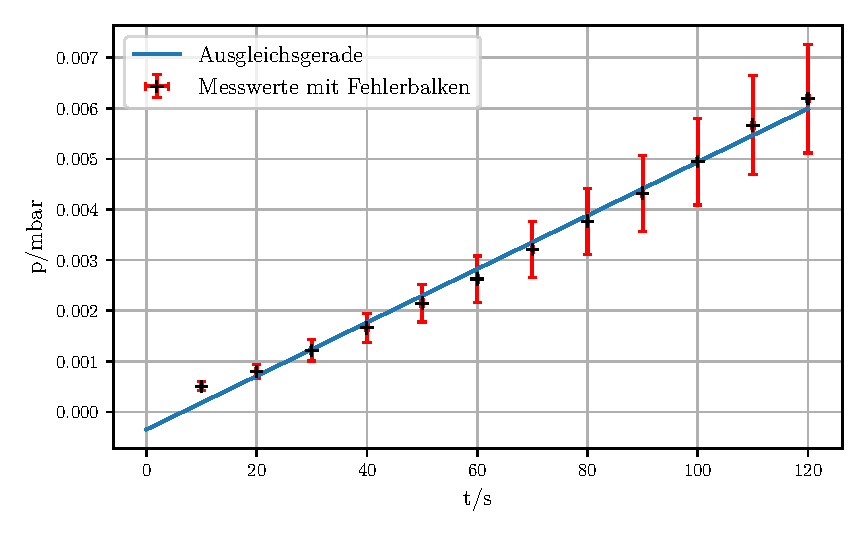
\includegraphics[width=0.8\textwidth]{abb/turbo_leck2e-4.pdf}
        \caption{Messergebnisse und Ausgleichsgeraden der Leckratenmessung zur Turbomolekularpumpe mit $p_g = \qty{2e-4}{\milli\bar}$.}
        \label{fig:turboLeck2}
    \end{figure}

    \begin{figure}
        \centering
        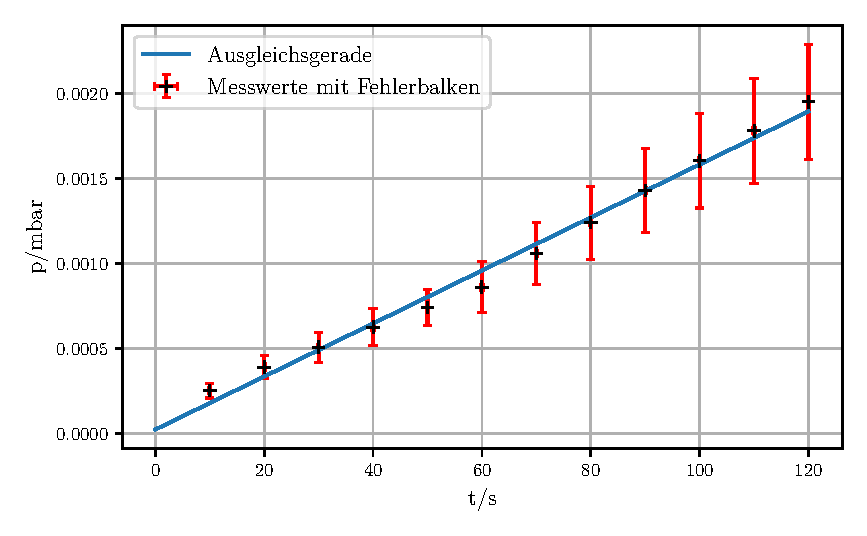
\includegraphics[width=0.8\textwidth]{abb/turbo_leck1e-4.pdf}
        \caption{Messergebnisse und Ausgleichsgeraden der Leckratenmessung zur Turbomolekularpumpe mit $p_g = \qty{1e-4}{\milli\bar}$.}
        \label{fig:turboLeck1}
    \end{figure}

    \begin{figure}
        \centering
        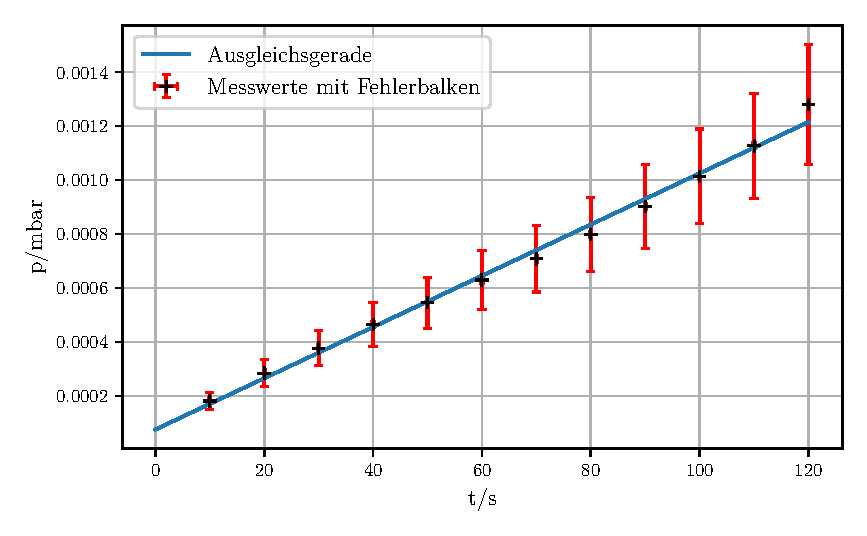
\includegraphics[width=0.8\textwidth]{abb/turbo_leck7e-5.pdf}
        \caption{Messergebnisse und Ausgleichsgeraden der Leckratenmessung zur Turbomolekularpumpe mit $p_g = \qty{7e-5}{\milli\bar}$.}
        \label{fig:turboLeck7}
    \end{figure}

    \begin{figure}
        \centering
        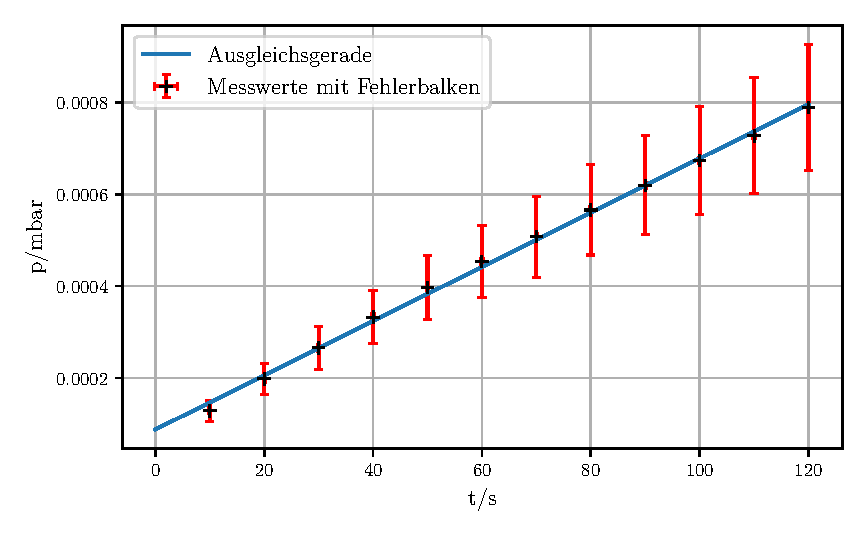
\includegraphics[width=0.8\textwidth]{abb/turbo_leck5e-5.pdf}
        \caption{Messergebnisse und Ausgleichsgeraden der Leckratenmessung zur Turbomolekularpumpe mit $p_g = \qty{5e-5}{\milli\bar}$.}
        \label{fig:turboLeck5}
    \end{figure}


